\documentclass[10pt]{beamer}

% Watch out for lines like
%% Mat kicks in
%% Luca kicks in
% in order to know which slides belong to whom

% Handout Generation {{{

% \documentclass[10pt,handout]{beamer}
% \usepackage{pgfpages}
% \pgfpagesuselayout{4 on 1}[a4paper, landscape, border shrink=5mm]
% \pgfpageslogicalpageoptions{1}{border code=\pgfusepath{stroke}}
% \pgfpageslogicalpageoptions{2}{border code=\pgfusepath{stroke}}
% \pgfpageslogicalpageoptions{3}{border code=\pgfusepath{stroke}}
% \pgfpageslogicalpageoptions{4}{border code=\pgfusepath{stroke}}

% Packages {{{1

\usepackage{graphicx}
\usepackage{xcolor}
\usepackage{tikz}
\usetikzlibrary{shapes}
\usepackage{ifthen}
\usepackage{fontspec}
\usepackage{fontawesome}
\newfontfamily{\FA}{FontAwesome}
\usepackage{verbatim}

\definecolor{KTHBlue}{HTML}{003C9E}
\definecolor{DarkGreen}{HTML}{526B0B}
\definecolor{DarkRed}{HTML}{AB2511}

% Theming {{{1
\usetheme[progressbar=foot]{metropolis}

\setbeamercolor{normal text}{%
	fg=black!90,
	bg=black!2
}
\setbeamercolor{alerted text}{%
	fg=KTHBlue!80,
	bg=black!2
}
\setbeamercolor{palette primary}{%
	use=normal text,
	fg=normal text.bg,
	bg=KTHBlue
}
\setbeamercolor{progress bar in head/foot}{fg=KTHBlue, bg=KTHBlue!10}
\setbeamercolor{progress bar in section page}{fg=KTHBlue, bg=KTHBlue!10}
\setbeamercolor{title separator}{fg=KTHBlue}

\AtBeginSubsection{\frame{\subsectionpage}}

%% Luca kicks in

% Title Page {{{1

\title{Coding: Best Practices \& Tools}
\subtitle{Towards painless programming for researchers}
\author{L. \textsc{Manzari} -- M. \textsc{Gaborit}}
\date{MWL Lunch Seminar -- June 1, 2016}
\institute{}
\titlegraphic{\hfill
\includegraphics[height=1.5cm]{logo}}

% Icons {{{1

\def\githubicon{{\FA\symbol{"F09B}} }
\def\giticon{{\FA\symbol{"F1D3}} }
\def\foldericon{{\FA\symbol{"F07C}} }
\def\zipicon{{\FA\symbol{"F1C6}} }

% Graphics {{{1

\newcommand\fileimage[1]{%
	\draw[fill=black!2] (#1) -- ++(2,0) -- ++(0,2.5) -- ++(-1.5,0) -- ++(-.5,-.5) -- cycle;
}

\newcommand\researchpaper[1]{
	\fileimage{#1};
	\foreach \i in {1,...,17} {
		\draw (#1) ++(.1,.1*\i) -- ++(.8,0) ++(.2,0) -- ++(.8,0);
	}
	% title
	\draw[thick] (#1) ++(.3,2.1) -- ++(1.4,0);
	\draw[thick] (#1) ++(.5,2.0) -- ++(1,0);
}


% }}}
\begin{document}

% Title and TOC {{{1
\maketitle

\begin{frame}{Contents}
	\setbeamertemplate{section in toc}[sections numbered]
	\tableofcontents[hideallsubsections]
\end{frame}

\section{Better practices in coding: why?} % {{{1

\begin{frame}{Better practices in coding: why?}

	\begin{quotation}
		Instead of imagining that our main task is to instruct a
		computer what to do, let us concentrate rather on explaining to human
		beings what we want a computer to do.
	\end{quotation}
	\begin{flushright}
		--- D. Knuth
	\end{flushright}

\end{frame}

\section{Editors \& IDEs} % {{{1

\begin{frame}{File types in research} % {{{2

	\begin{center}
		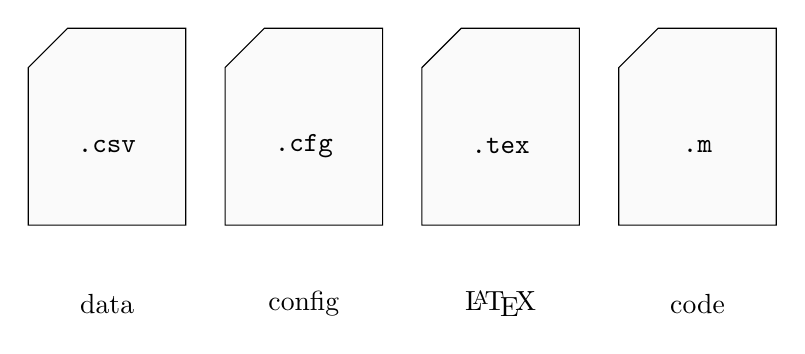
\begin{tikzpicture}
			\foreach \t/\e [count=\i] in {data/.csv,config/.cfg,\LaTeX{}/.tex,code/.m}{
				\pause
				\fileimage{2.5*\i,0};
				\node (tmp) at (2.5*\i+1,-1) {\t};
				\node (tmp) at (2.5*\i+1,1) {\textbf{\texttt{\e}} };
			}
		\end{tikzpicture}
		\pause{}

		\uncover<6,7>{
			\Large
			These are all \alert{text files}...
		}

		\uncover<7>{
			...let's use \alert{a good text editor}!
		}
	\end{center}
\end{frame}

\begin{frame}{What makes a text editor \emph{good}?} % {{{2

	\large
	A good text editor has to be...
		\begin{itemize}
			\item Invisible
			\item Intelligent
			\item Customizable
			\item Extensible
		\end{itemize}

\end{frame}

\begin{frame}{All the fuss about VIm and GNU Emacs} % {{{2

	\large
	\begin{description}
		\item[Pros]
			\begin{itemize}
				\item learn once, use forever
				\item available everywhere
				\item (im)proved with time
			\end{itemize}
		\item[Cons]
			\begin{itemize}
				\item at the beginning, intimidating
			\end{itemize}
	\end{description}

\end{frame}

\begin{frame}{Editors: GNU Emacs} % {{{2
	\large
	\begin{block}{Characteristics}
		\begin{itemize}
			\item It's not a text editor, it's a Lisp interpreter
			\item Highly context-dependent behavior
		\end{itemize}
	\end{block}
	\uncover<2>{
			\begin{block}{How to get started}
				\begin{enumerate}
					\item use it as a regular text editor
					\item customize according to need
					\item extend it using packages
				\end{enumerate}
			\end{block}
	}

\end{frame}

%% Mat kicks in

\begin{frame}{Editors: VIm} % {{{2
	\only<1>{
		\begin{block}{What people think it is...}
			\begin{center}
				
\includegraphics[width=.9\textwidth]{images/vim/people_think.png}
			\end{center}
		\end{block}
	}
	\only<2>{
		\begin{block}{What it does actually look like}
			\begin{center}
			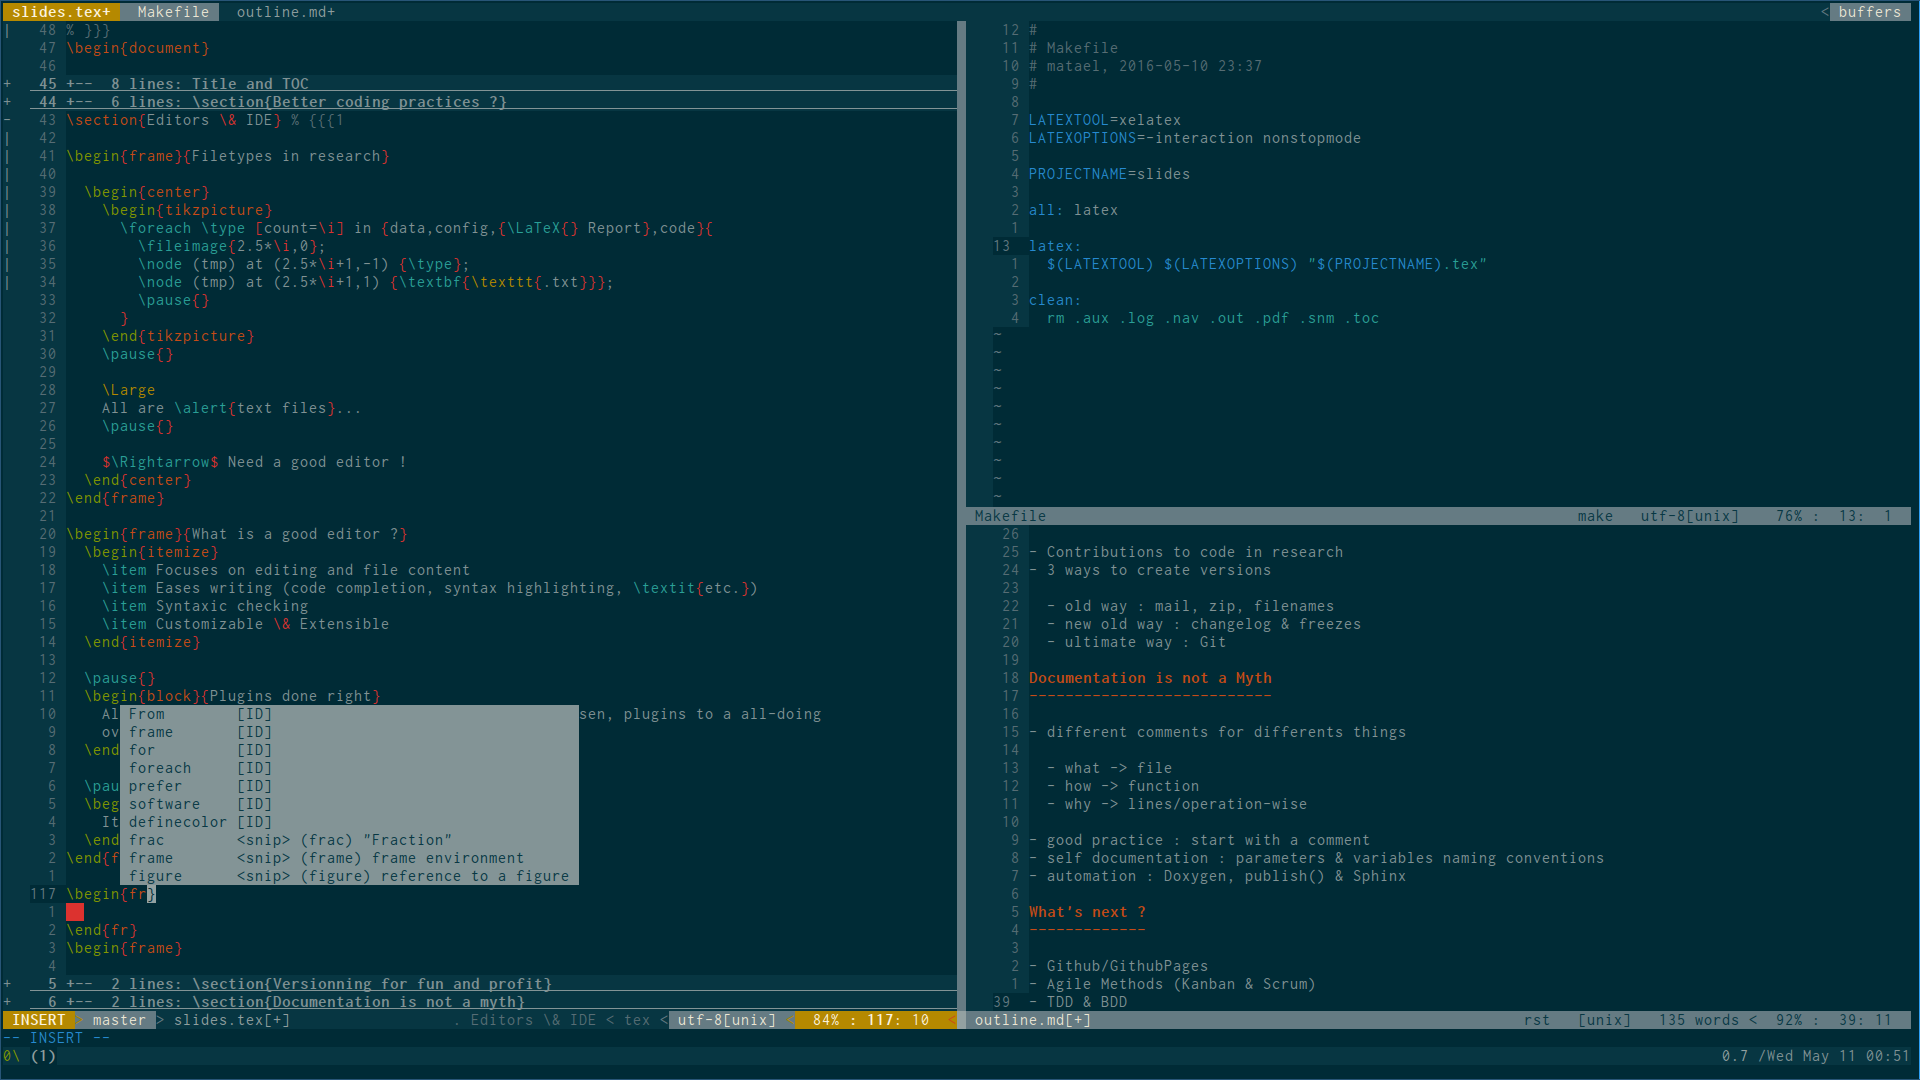
\includegraphics[width=.9\textwidth]{images/vim/actual.png}
			\end{center}
		\end{block}
	}
	\only<3>{
		\begin{block}{Characteristics}
			\begin{itemize}
				\item Command line or GUI
				\item Modal (one mode per class of action: edition, displacement, selection, etc...)
				\item Based on shortcuts and commands
				\item Fully customizable through plugin or embedded language
				\item Painless integration with any standard UNIX toolchain
			\end{itemize}
		\end{block}
		\begin{block}{Where to start}
			\begin{itemize}
				\item \url{http://vim-adventures.com/} \& \texttt{\$ vimtutor}
				\item \url{http://vimcasts.org/}
				\item \url{https://vimebook.com/en}
			\end{itemize}
		\end{block}
	}
\end{frame}


\begin{frame}{Editors: for the fainthearted} % {{{2
	\large
	Multi-platform, open-source and actively maintained

	\medskip

	\begin{itemize}
		\item \textbf{Atom} \hfill \url{atom.io}
		\item \textbf{Light Table} \hfill \url{lighttable.com}
		\item \textbf{Sublime Text} \hfill \url{sublimetext.com}
	\end{itemize}

\end{frame}
% }}}

\section{Versioning for fun and profit} % {{{1

\begin{frame}{Contribution to a research code} % {{{2
	\begin{center}
		\begin{tikzpicture}[>=stealth, scale=.8, transform shape]
			% central node
			\node[KTHBlue] (researchcode) at (0,0) {\textbf{Research Code}};
			\draw[KTHBlue, line width=.5mm] (0,0) ellipse (1.7 and .7);

			% team
			\newcommand\teammember[1]{%
				\fill[black] (#1) -- ++(.3,0) .. controls ++(0,.15) and ++(.1,0) .. ++(-.15,.3) .. controls ++(-.1,0) and ++(0,.15) .. (#1);
				\fill[black] (#1) ++(.15,.37) circle (.07);
			}

			\foreach \x/\y in {-6/3, -4.5/3, -4/1.5, -5.5/1.5}{
				\teammember{\x,\y};
			}
			\draw[dashed, line width=.5mm] (-4.9,2.5) circle (1.7) node{Team};
			\draw[->, line width=.5mm] (-4.9,2.5) ++(-10:2) .. controls ++(.8,-.3) and ++(-.3,.6) ..  (160:1.6);

			% Publications
			\begin{scope}[xscale=-1]
				\draw[<-, line width=.5mm] (-4.9,-.6) ++(40:2.3) .. controls ++(.7,.4) and ++(-.4,.5) ..  (160:1.6);
			\end{scope}

			\foreach \j in {0,...,2} {
				\researchpaper{3.5+\j*.6,1.4-.4*\j};
			}
			\node (tmp) at (5,4.2) {Publications};


			% partners
			\begin{scope}[shift={(-3,0)}]
				\draw[thick] (-3,-5) -- ++(7,0) node[midway, below] {Academic \& Industrial Partners};
				\begin{scope}[shift={(2,1)}, rotate=70]
					\draw[<->, line width=.5mm] (-4.9,-.6) ++(40:2.3) .. controls ++(.7,.4) and ++(-.4,.5) ..  (160:1.6);
				\end{scope}

				% academic partner
				\draw[thick] (-2.5,-5) rectangle ++(2.2,2.8);
				\foreach \i in {0,...,3} {
					\foreach \j in {0,...,2} {
						\draw (-2.3+\j*.7,-4.3+\i*.5) rectangle ++(.4,.4);
					}
				}
				\draw (-2.3,-4.8) rectangle ++(.4,.4);
				\draw (-2.3+2*.7,-4.8) rectangle ++(.4,.4);
				\draw (-1.7,-5) rectangle ++(.3,.6);
				\draw (-1.4,-5) rectangle ++(.3,.6);

				% indus
				\draw[thick] (1,-5) --++(0,1.3)
				-- ++(.7,-.5) --++(0,.5)
				-- ++(.7,-.5) --++(0,.5)
				-- ++(.7,-.5) --++(0,1) --++(.5,0) -- ++(0,-1.8) -- cycle;
			\end{scope}

			% release

			\node (gh) at (4,-2) {\Huge\githubicon};
			\node (tmp) at (4,-3) {Public Release};
			\draw[->, line width=.5mm] (-20:1.6) .. controls ++(.8,0) and ++(-.6,.7) .. (3.6, -1.5);
		\end{tikzpicture}
	\end{center}
\end{frame}

% }}}
\begin{frame}{Versioning} % {{{2
	\begin{center}
		\only<1>{We need to \textbf{\alert{edit}} files every single day.}
		\only<2>{We need to \textbf{\alert{collaborate on}} files every single day.}
		\only<3>{We need to \textbf{\alert{review}} files every single day.}
		\only<4>{We need to \textbf{\alert{explore}} files every single day.}
		\only<5>{We need to \textbf{\alert{share}} files every single day.}

		\only<6>{\Large{We need a reliable versioning system!}}
	\end{center}
\end{frame}

% }}}

\subsection{The old old way : name it, zip it, mail it} % {{{2

\begin{frame}{Versioning: the old old way} % {{{3
	The first versioning attempts traditionally rely on 3 pillars:

	\begin{itemize}
		\item Naming conventions
		\item Regular backups
		\item Careful data management
	\end{itemize}

	\pause
	\medskip

	\begin{center}
		\alert{\Large{``C'mon, I even mailed myself the latest version:\\how could this go wrong?''}}
	\end{center}

\end{frame}

\begin{frame}{Versioning: the old old way} % {{{3

	\begin{center}
		\begin{tikzpicture}[scale=1]
			\foreach [evaluate={\remainder=Mod(\i,2)}] \name/\icon [count=\i] in
			{Awesome\_project/\foldericon, Awesome\_project\_2/\foldericon,
			Awesome\_project\_backup/\zipicon, Awesome\_project\_test/\foldericon,
			Awesome\_project\_test\2/\foldericon, Awesome\_project\_backup\_2/\zipicon,
			Awesome\_project\_idea\_sunday/\foldericon, Awesome\_project\_publi/\foldericon,
			Awesome\_project\_publi\_fix/\foldericon, Awesome\_project\_not\_good/\foldericon,
			{...}/{~~~} } {
				\ifthenelse{\remainder=1}{
					\draw[black!8, fill=black!8] (0,-.5*\i) rectangle ++(9,.5);
				}{
					\draw[black!5, fill=black!5] (0,-.5*\i) rectangle ++(9,.5);
				}
				\node[anchor=west] (tmp) at (0,.2-.5*\i) {\icon~~\name};
				\pause{}
			}
		\end{tikzpicture}
	\end{center}
\end{frame}

\begin{frame}{Versioning: the old old way} % {{{3

	Plus, this does not behave well when scaling things up...

	\begin{itemize}
		\item How to handle team-work?
		\item Modification conflicts: what to do?
		\item No continuous time travel
		\item ...and a lot more issues
	\end{itemize}

\end{frame}


\subsection{The new old way : \{Drop,\}Box and Changelogs} % {{{2

\begin{frame}{Versioning: the new old way} % {{{3

	The Cloud: one more step towards real-time collaboration!

	\begin{itemize}
		\item Free \& paid plans
		\item Auto-sync even for big files
		\item Team notifications
		\item Mobile access to files
		\item A carefully maintained changelog \emph{may} keep track of changes
	\end{itemize}

	\pause
	But...
	\pause
	does the "Cloud" really share the spirit that drives research?

\end{frame}

\begin{frame}{Terms of Service: chosen moments} % {{{3

	\only<1>{
		\begin{quotation}
			These and other features may require our systems
			to \textbf{\alert{access, store and scan}} Your Stuff.
		\begin{flushright}
			--- DropBox TOS
		\end{flushright}
		\end{quotation}
	}
	\only<2>{
		\begin{quotation}
			You hereby grant Box and its contractors the
			right to \textbf{\alert{transmit, use and disclose}}
			Content posted on the Service solely to the
			extent necessary to provide the Service, as
			otherwise permitted by these Terms, or to
			\textbf{\alert{comply with any request}} of a
			governmental or regulatory body (including
			subpoenas or court orders)
		\begin{flushright}
			--- Box TOS
		\end{flushright}
		\end{quotation}
	}
	\only<4>{
		What about iCloud?

		\begin{quotation}
			Apple reserves the right at all times to
			determine whether Content is appropriate and in
			compliance with this Agreement, and may
			pre-screen, \textbf{\alert{move, refuse, modify and/or remove}} Content at any time,
			without prior notice and in its sole discretion [\ldots]
		\begin{flushright}
			--- iCloud TOS
		\end{flushright}
		\end{quotation}

	}
	\only<5>{
		What about iCloud?

		\begin{quotation}
			However, by submitting or posting such Content
			on areas of the Service that are accessible by
			the public or other users with whom you consent
			to share such Content, you grant Apple a
			worldwide, royalty-free, non-exclusive license
			to \textbf{\alert{use, distribute, reproduce, modify, adapt, publish, translate, publicly perform and publicly display}} such
			Content on the Service solely for the purpose
			for which such Content was submitted or made
			available, without any compensation or
			obligation to you.
		\begin{flushright}
			--- iCloud TOS
		\end{flushright}
		\end{quotation}
	}

	\only<3>{
		\begin{quotation}
			When you upload, submit, store, send or receive
			content to or through our Services, you give
			Google (and those we work with) a worldwide
			license to \textbf{\alert{use, host, store, reproduce, modify, create derivative works, communicate, publish, publicly perform, publicly display and distribute}} such
			content. [...] This license continues even if
			you stop using our Services [...]
		\begin{flushright}
			--- Google TOS
		\end{flushright}
		\end{quotation}
	}
\end{frame}

\subsection{The badass way: \giticon} % {{{2

	\begin{frame}{Versioning: the badass way} % {{{3

		\giticon was built to handle huge projects, like the Linux kernel:

		\begin{itemize}
			\item distributed (everyone has a full copy)
			\item efficient (only changes are transferred)
			\item commit-wise versioning
			\item supporting branches (new ideas in a enclosed space) and tagging
			\item potentially server-less \& self-hostable
			\item simultaneous modifications \& smart merging
			\item usable through GUI (tig, gitk, tortoise-git \& others) or command-line
		\end{itemize}

	\end{frame}

	\begin{frame}{Versioning: the badass way} % {{{3

		Concerning commits...

		\begin{center}
			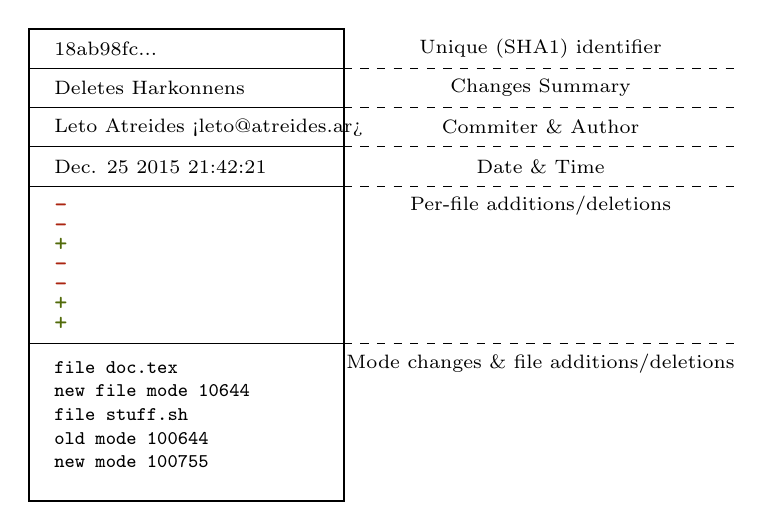
\begin{tikzpicture}
				\draw[thick] (0,0) rectangle ++(4,6);

				\draw (0,5.5) -- ++(4,0);
				\node[anchor=west] (tmp) at (.2,5.75) {\scriptsize{18ab98fc...}};
				\draw (0,5) -- ++(4,0);
				\node[anchor=west] (tmp) at (.2,5.25) {\scriptsize{Deletes Harkonnens}};
				\draw (0,4.5) -- ++(4,0);
				\node[anchor=west] (tmp) at (.2,4.75) {\scriptsize{Leto Atreides <leto@atreides.ar>}};
				\draw (0,4) -- ++(4,0);
				\node[anchor=west] (tmp) at (.2,4.25) {\scriptsize{Dec. 25 2015 21:42:21}};
				\draw (0,2) -- ++(4,0);
				\foreach \sign/\col [count=\i] in { +/DarkGreen, +/DarkGreen, -/DarkRed, -/DarkRed, +/DarkGreen, -/DarkRed, -/DarkRed} {
					\node[anchor=west, color=\col] (tmp) at (.2,2+.25*\i) {\textbf{\small{\texttt{\sign}} }};
				}
				\foreach \mode [count=\i] in { file doc.tex, new file mode 10644, file stuff.sh, old mode 100644,  new mode 100755 } {
					\node[anchor=west] (tmp) at (.2,2-.3*\i) {\scriptsize{\texttt{\mode}} };
				}

				% explanations
				\foreach \hght in {5, 5.5, 4.5, 4, 2} {\draw[dashed] (4,\hght) -- ++(5,0);}

				\foreach \hght/\text in {
					{5+.75/Unique (SHA1) identifier},
					{5+.25/Changes Summary},
					{4.5+.25/Commiter \& Author},
					{4+.25/Date \& Time},
					{4-.25/{Per-file additions/deletions}},
					{2-.25/{Mode changes \& file additions/deletions}},
				}{
					\node (tmp) at (6.5,\hght) {\scriptsize{\text}};
				}
			\end{tikzpicture}

			All the needed information is here!
		\end{center}
	\end{frame}

	\begin{frame}{Versioning: the badass way} % {{{3
		\begin{center}
			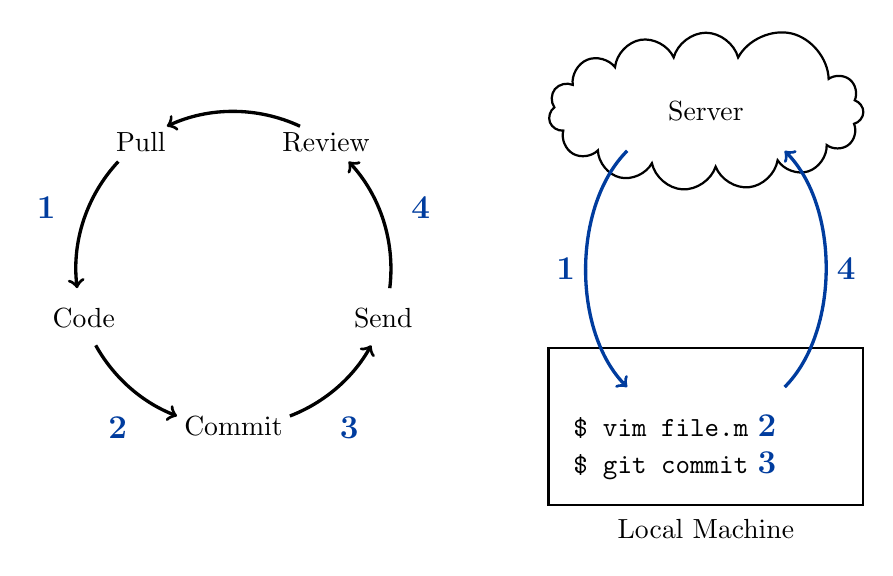
\begin{tikzpicture}
				\foreach \step/\stepcount/\corrb/\corra [count=\i] in {Pull/1/0/0, Code/2/0/10, Commit/3/10/0, Send/4/0/0, Review//0/0} {
					\node (tmp) at (-36+\i*72+90:2) {\step};
					\node[KTHBlue] (tmp) at (\i*72+90:2.5) {\large{\textbf{\stepcount}} };
					\draw[->, very thick] (-25+\i*72+90+\corrb:2) arc (-25+\i*72+90+\corrb:25+\i*72+90-\corra:2);
				}

				\node[cloud, thick, cloud puffs=14.7, cloud ignores aspect, minimum width=4cm, minimum height=2cm, align=center, draw] (cloud) at (6,2) {Server};
				\draw[thick] (4,-3) rectangle ++(4,2);
				\node (tmp) at (6,-3.3) {Local Machine};

				\draw[KTHBlue, ->, very thick] (5,1.5) .. controls ++(-.7,-.7) and ++(-.7,.7) ..  (5,-1.5) node[midway, left] {\large{\textbf{1}} };
				\draw[KTHBlue, <-, very thick] (7,1.5) .. controls ++(.7,-.7) and ++(.7,.7) ..
				(7,-1.5) node[midway, right] {\large{\textbf{4}} };

				\node[anchor=west] (tmp) at (4.2,-2) {\texttt{\$ vim file.m} \textcolor{KTHBlue}{\large{\textbf{2}} }};
				\node[anchor=west] (tmp) at (4.2,-2.5) {\texttt{\$ git commit} \textcolor{KTHBlue}{\large{\textbf{3}} }};

			\end{tikzpicture}
		\end{center}
	\end{frame}

	\begin{frame}{Versioning: the badass way} % {{{3

		\begin{center}
			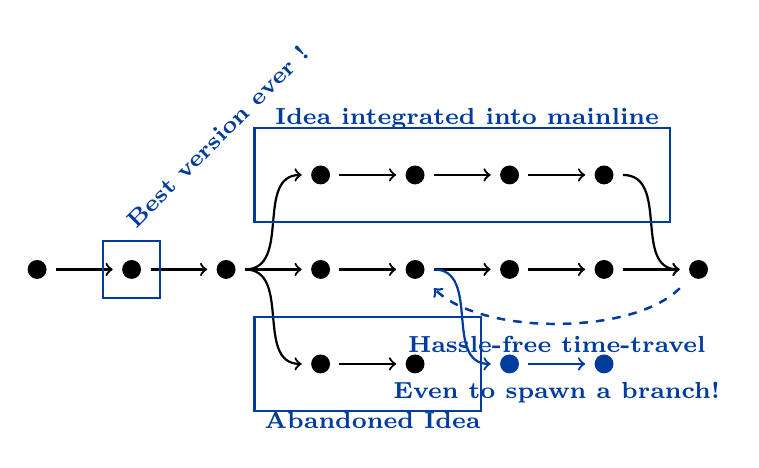
\begin{tikzpicture}[scale=1.2, transform shape]

				% dots
				\foreach \x/\y in {
					0/0, 1/0, 2/0, 3/0, 4/0, 5/0, 6/0, 7/0,
					3/1, 4/1, 5/1,	6/1,
					3/-1, 4/-1 } {
					\fill[black](\x,\y) circle (.1);
				}

				% straight arrows
				\foreach \x/\y in {
					0/0, 1/0, 2/0, 3/0, 4/0, 5/0, 6/0,
					3/1, 4/1, 5/1,
					3/-1 } {
					\draw[->, thick] (\x+.2,\y) -- (\x+.8,\y);
				}

				% branching
				\draw[->, thick] (2.2,0) .. controls ++(.5,0) and ++(-.5,0) .. (2.8,1);
				\draw[->, thick] (6.2,1) .. controls ++(.5,0) and ++(-.5,0) .. (6.8,0);
				\draw[->, thick] (2.2,0) .. controls ++(.5,0) and ++(-.5,0) .. (2.8,-1);

				% interaction
				%% tags
				\uncover<2>{
					\draw[thick, KTHBlue](.7,-.3) rectangle ++(.6,.6);
					\node[KTHBlue, rotate=45,anchor=west] (tags) at (.9,.4) {\textbf{\scriptsize{Best version ever !}} };
				}
				\uncover<3>{
					\draw[KTHBlue, thick] (2.3,.5) rectangle (6.7,1.5);
					\node[KTHBlue] (merged_branch) at (4.55,1.6) {\textbf{\scriptsize{Idea integrated into mainline}} };
				}
				\uncover<4>{
					\draw[KTHBlue, thick] (2.3,-.5) rectangle (4.7,-1.5);
					\node[KTHBlue] (cancelled_branch) at (3.55,-1.6) {\textbf{\scriptsize{Abandoned Idea}} };
				}
				\uncover<5>{
					\draw[KTHBlue, dashed, thick, ->] (6.8,-.2) .. controls ++(-.5,-.5) and ++(.5,-.5) ..
					(4.2,-.2) node[midway, below] {\textbf{\scriptsize{Hassle-free time-travel}} };
				}
				\uncover<6>{
					\draw[KTHBlue, dashed, thick, ->] (6.8,-.2) .. controls ++(-.5,-.5) and ++(.5,-.5) .. (4.2,-.2);
					\fill[KTHBlue](5,-1) circle (.1);
					\fill[KTHBlue](6,-1) circle (.1);

					\draw[KTHBlue, ->, thick] (5+.2,-1) -- ++(.6,0);
					\draw[KTHBlue, ->, thick] (4.2,0) .. controls ++(.5,0) and ++(-.5,0) .. (4.8,-1);

					\node[KTHBlue] (branching) at (5.5,-1.3) {\textbf{\scriptsize{Even to spawn a branch!}} };
				}
			\end{tikzpicture}
		\end{center}
	\end{frame}

	% }}}

% }}}

%% Luca kicks in

\section{Documentation} % {{{1

\begin{frame}{Documentation} % {{{2
	\begin{center}
		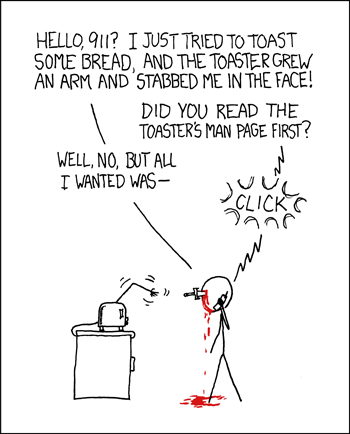
\includegraphics[height=.85\textheight]{images/docs/rtfm.png}
	\end{center}
	{\tiny Courtesy of Randall Munroe, https://xkcd.com/293}
\end{frame}

\begin{frame}{Documentation: why} % {{{2

	\large
	Before using a program, it's good to know:

	\begin{itemize}
		\item \textbf{what} it does
		\item \textbf{how} it does it
		\item \textbf{why} it does it like that
	\end{itemize}

	\bigskip

	\uncover<2>{
		Code tells you \textbf{how}.

	Documentation tells you the rest.
	}

\end{frame}

\begin{frame}{Documentation: types} % {{{2

	\large
	\begin{block}{Internal}
		\begin{itemize}
			\item comments
			\item self-documenting code
		\end{itemize}
	\end{block}

	\bigskip

	\begin{block}{External}
		\begin{itemize}
			\item separate manual
			\item referenced material
		\end{itemize}
	\end{block}

\end{frame}

\section{Internal documentation} % {{{1

\begin{frame}[fragile]{Internal documentation: comments} % {{{2

	\begin{block}{Begin every file with a comment}
		\begin{itemize}
			\item say what the code should do
			\item describe how to use the file
		\end{itemize}
	\end{block}

	\begin{block}{A MATLAB example}
\begin{verbatim}
function [h,a] = pythagoras(c1,c2)
% pythagoras -- computes the hypotenuse and the area of a
%               right-angled triangle
%
% Inputs: c1 - length of the first cathetus [m]
%         c2 - length of the second cathetus [m]
% Outputs: h - length of the hypotenuse [m]
%          a - area of the triangle [m^2]
%
% Example: [hypo,area] = pythagoras(3,4)
\end{verbatim}
	\end{block}

\end{frame}

\begin{frame}{Internal documentation: comments} % {{{2
	\large
	\begin{itemize}
		\item Explain \textbf{why}
		\item Close to code they refer to
		\item If updating the code, \textbf{update the comments}
		\item Avoid them if unnecessary
	\end{itemize}

\end{frame}

\begin{frame}[fragile]{Internal documentation: comments} % {{{2

	\begin{block}{What is ``unnecessary''}
		What feels obvious to you when writing the code may not be
		obvious to someone else, or even to you at a future time.
	\end{block}

	\begin{block}{A MATLAB example}
\begin{verbatim}
%   ** USELESS COMMENT **
% compute the mean value of every column of A
B = mean(A,1);

%   ** USEFUL, bsxfun may be obscure! **
% divide every column of A by the column vector v
B = bsxfun(@rdivide,A,v);
\end{verbatim}
	\end{block}

\end{frame}

\begin{frame}[fragile]{Internal documentation: comments} % {{{2
	\large
	\begin{block}{When commenting...}
		\begin{itemize}
			\item ...a library, say \alert{\textbf{what}} it does
\begin{verbatim}
% This toolbox computes PSDs.
\end{verbatim}
			\item ...a function, say \alert{\textbf{how}} it does it
\begin{verbatim}
% PSD estimate using Welch's method.
\end{verbatim}
			\item ...a line, say \alert{\textbf{why}} it does it that way
\begin{verbatim}
\% bsxfun is faster than a for loop
\end{verbatim}
		\end{itemize}
	\end{block}
\end{frame}

\begin{frame}{Internal documentation: self-documenting code} % {{{2

	\large
	\begin{quotation}
		Programs must be written for people to read, \\ and only
		incidentally for machines to execute.
		\begin{flushright}
			--- Structure and interpretation\\of computer programs
		\end{flushright}
	\end{quotation}

	\bigskip

	\begin{itemize}
		\item Aim at writing code that does not need comments
		\item Use meaningful, non-ambiguous variable names
	\end{itemize}

\end{frame}

\section{External documentation} % {{{1

\begin{frame}{External documentation} % {{{2

	Quality internal documentation can be used to automatically
	generate external documentation.

	\begin{block}{A MATLAB example}
		\begin{description}
			\item[publish()] code publishing tool included in MATLAB
		\end{description}
	\end{block}

	\begin{block}{More useful tools}
		\begin{description}
			\item[Doxygen] doc-generator supporting multiple languages
			\item[Sphinx] doc-generator built for the Python project
			\item[rtfd.org] free web-service for hosting documentation
		\end{description}
	\end{block}

\end{frame}

%% Mat kicks in

\section{What's next?} % {{{1

\begin{frame}{Cut scenes}
		We couldn't fit it all in... so here is the rest:

		\begin{description}
			\item[Github] Public Git server for free software (paid plans exist)
				with webpage publishing service (good to host the homepage of a project).
			\item[Agility] Project management methods centered on human relations more than on
				tools and processes. See Kanban or Scrum for an introduction.
			\item[TDD \& BDD] Test- \& Behavior Driven Development. Coding paradigms focusing
				on certain aspects (reliability \& spec. compliance). Useful to scale from a
				research PoC to a distributed software.
		\end{description}
\end{frame}


\begin{frame}[standout] % Thank you {{{1
	% Thank you!\\
	\vspace{0.05\textwidth}
	% It really looks like the BSOD, lol
	\colorbox{white}{\textcolor{KTHBlue}{Questions?}}\\
	\vspace{0.25\textwidth}
	\scriptsize{\texttt{manzari@kth.se}} --- \scriptsize{\texttt{gaborit@kth.se}}\\
\end{frame}

%}}}
\end{document}
